\documentclass{standalone}

\usepackage[dvipsnames]{xcolor}
\usepackage{tikz}

\usepackage{booktabs}

\usepackage{fontspec}
\setmainfont{Tex Gyre Schola}

\usepackage{array}
%\renewcommand{\arraystretch}{2}
\begin{document}

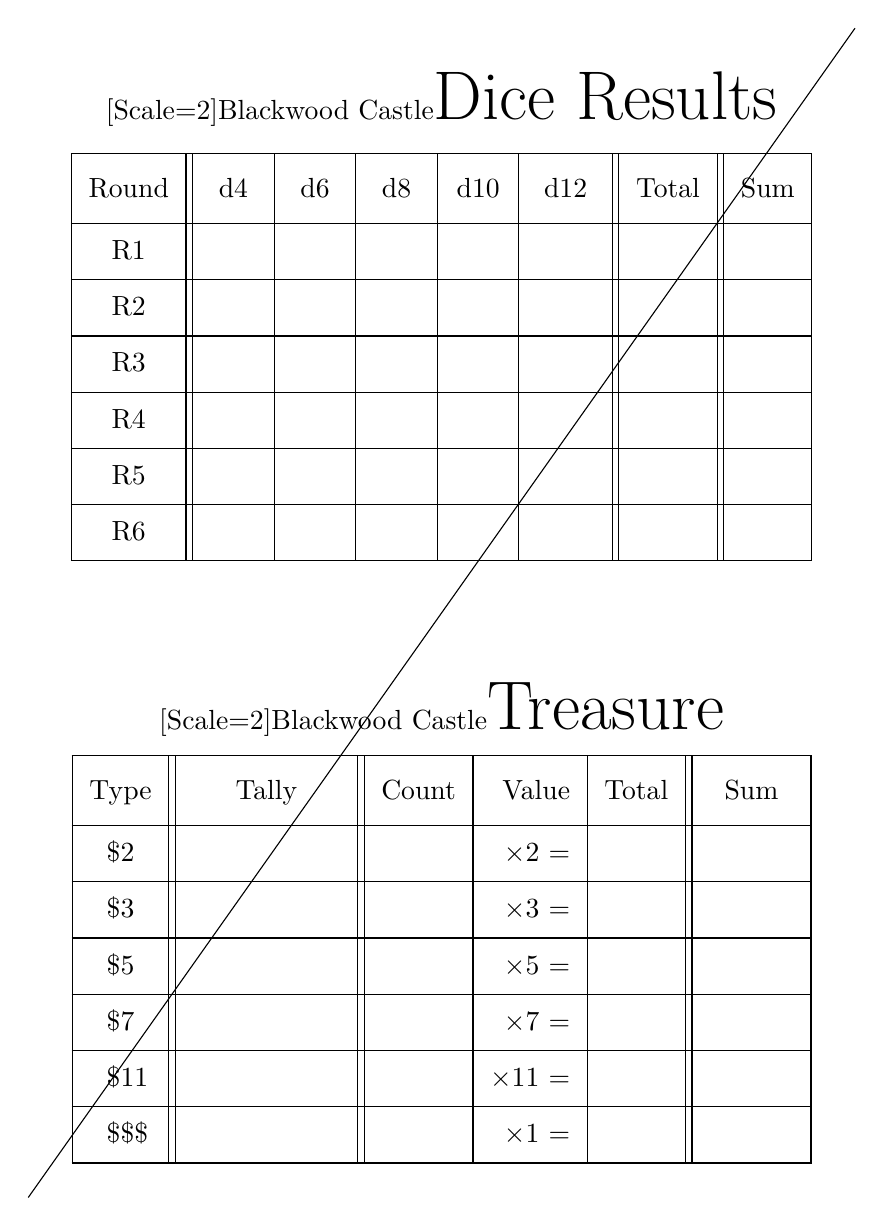
\begin{tikzpicture}
\path[draw] (-52.5mm,-74.25mm) -- (52.5mm, 74.25mm);
%\path[draw] (-52.5mm, -37.125mm) -- (52.5mm, 37.125mm);

\node[anchor=north] at (0,70mm) {
\begin{tabular}{|c||m{6mm}|m{6mm}|m{6mm}|m{6mm}|m{7.5mm}||c||c|}%||rrrrrl|l|}
\multicolumn{8}{c}{\setmainfont[Scale=2]{Blackwood Castle}\Huge Dice Results} \\[3mm]\hline
Round\raisebox{-2.5mm}{\rule{0mm}{8mm}} & \centering d4 & \centering d6 & \centering d8 & \centering d10 & \centering d12 & Total & Sum\\[2mm]\hline 
R1\raisebox{-2.5mm}{\rule{0mm}{7mm}} & & & & & & & \\\hline%% & & & & & & &\\
R2\raisebox{-2.5mm}{\rule{0mm}{7mm}} & & & & & & & \\\hline
R3\raisebox{-2.5mm}{\rule{0mm}{7mm}} & & & & & & & \\\hline
R4\raisebox{-2.5mm}{\rule{0mm}{7mm}} & & & & & & & \\\hline
R5\raisebox{-2.5mm}{\rule{0mm}{7mm}} & & & & & & & \\\hline
R6\raisebox{-2.5mm}{\rule{0mm}{7mm}} & & & & & & & \\\hline
\end{tabular}
};



\node[anchor=south, inner sep=0pt] at (0,-70mm) {
\begin{tabular}{|c||m{18.75mm}||c|r|c||c|}%||rrrrrl|l|}
\multicolumn{6}{c}{\setmainfont[Scale=2]{Blackwood Castle}\Huge Treasure} \\[2mm]\hline
Type\raisebox{-2.5mm}{\rule{0mm}{8mm}} & \centering Tally & Count & \centering Value & Total & \phantom{S}Sum\phantom{S}\\[2mm]\hline 
\$2\raisebox{-2.5mm}{\rule{0mm}{7mm}} & & & \raggedleft \times 2 = & & \\\hline
\$3\raisebox{-2.5mm}{\rule{0mm}{7mm}} & & & \raggedleft \times 3 = & & \\\hline
\$5\raisebox{-2.5mm}{\rule{0mm}{7mm}} & & & \raggedleft \times 5 = & & \\\hline
\$7\raisebox{-2.5mm}{\rule{0mm}{7mm}} & & & \raggedleft \times 7 = & & \\\hline
\phantom{1}\$11\raisebox{-2.5mm}{\rule{0mm}{7mm}} & & & \raggedleft \times 11 = & & \\\hline
\phantom{\$}\$\$\$\raisebox{-2.5mm}{\rule{0mm}{7mm}} & & & \raggedleft \times 1 = & & \\\hline%% & & & & & & &\\
\end{tabular}
};

\end{tikzpicture}
\end{document}